\ifdefined \buildingFullOPALManual \else


%\ifx \@buildingFullOPALManual \@empty
%\else

%\documentclass[12pt,a4paper]{report}
\documentclass[a4paper]{book}

%% does not work in Latex2Html mode
%\usepackage{hyperref}

\usepackage[T1]{fontenc}
\usepackage{url}
\usepackage{html}
\usepackage{epic}
\usepackage{eepic}
\usepackage{makeidx}
\usepackage{array}
\usepackage{times}
\usepackage{amsmath}
\usepackage{amsxtra}
\usepackage{bm}
\usepackage[thin,thinp,thinc]{esdiff}
\usepackage{graphicx}
\usepackage{dingbat}
\usepackage{color}
\usepackage{subfig}
\usepackage{boxedminipage}
\usepackage{alltt}
\usepackage{nicefrac}
\usepackage{calc}
%\usepackage{pdfdraftcopy}             % Draft
\usepackage{tikz}
\usetikzlibrary{
  er,3d,calc,fadings,trees,positioning,arrows,chains,decorations.pathreplacing,
  decorations.pathmorphing,shapes,shapes.symbols,shapes.arrows,matrix,through,decorations.text
}

\tikzset{
  >=stealth',
  punktchain/.style={rectangle,rounded corners, draw=black, very thick,text width=10em,
                     minimum height=3em, text centered, on chain},
  line/.style={draw, thick, <-},
  element/.style={tape,top color=white,bottom color=blue!50!black!60!,minimum width=8em,
                  draw=blue!40!black!90, very thick,text width=10em, minimum height=3.5em,
                  text centered, on chain},
  every join/.style={->, thick,shorten >=1pt},
  tuborg/.style={decorate},
  tubnode/.style={midway, right=2pt}
}

\tikzstyle{material}=[draw, fill=blue!20, text width=16.0em, text centered, minimum height=1.5em]
\tikzstyle{diagramstep} = [material, text width=20em, minimum width=10em, minimum height=3em, rounded corners]
\tikzstyle{line} = [draw, thick, color=black!50, -latex']

\usepackage{booktabs}
\usepackage{xspace}
\usepackage{xstring}

\usepackage{fancyvrb}
\usepackage{rotating}
\usepackage{float}

\usepackage{tabularx}
\usepackage{longtable}
\setcounter{LTchunksize}{3}

\usepackage[section]{placeins}
\usepackage{MnSymbol}
\usepackage{microtype}
\usepackage{setspace}
\usepackage{dcolumn}

\usepackage[vmargin={3.0cm,3.0cm},
            hmargin={2.0cm,3.0cm}]{geometry}

\usepackage{upgreek}
\usepackage[binary-units=true]{siunitx}
\sisetup{exponent-product = \cdot,math-ohm=\Upomega,text-ohm=\ensuremath{\Upomega}}
\DeclareSIUnit{\clight}{c}
\DeclareSIUnit\gauss{Ga}

\usepackage{engord}
\usepackage{wasysym}
\DeclareSIUnit[number-unit-product = \,]{\permill}{\permil}

\usepackage{hyperref}
\hypersetup{
    pdftitle          = The OPAL Framework,
    pdfauthor         = {Andreas Adelmann, Achim Gsell, Valeria Rizzoglio, Christof Metzger-Kraus,
                         Yves Ineichen, Xiaoying Pang, Steve Russell, Chuan Wang, Jianjun Yang,
                         Suzanne Sheehy, Chris Rogers, Daniel Winklehner},
    pdfsubject        = User's Reference Manual,
    pdffitwindow      = true,               % page fit to window when opened
    pdfnewwindow      = true,               % links in new window
    colorlinks        = true,               % false: boxed links; true: colored links
    linkcolor         = black!80!green,     % color of internal links
    citecolor         = black!20!red,       % color of links to bibliography
    urlcolor          = blue,               % color of external links
    breaklinks        = true,
    bookmarksnumbered = true,
    plainpages        = false
}

\usepackage{ifthen}

\newif \iflinuxwindows
\linuxwindowstrue   % set this to true when building the manual on Linux or Windows
\iflinuxwindows
\usepackage{epstopdf}
\fi

\usepackage[backend=biber,
            style=phys,
            biblabel=brackets,
            maxnames=3,
            doi=true,
            isbn=true,
            url=true]{biblatex}
%---- macros ----

\renewcommand{\topfraction}{1.0}
\renewcommand{\bottomfraction}{1.0}
\renewcommand{\textfraction}{0.0}
\renewcommand{\arraystretch}{2.0}
\newenvironment{tex2html_nowrap}{}{}


\newcommand{\Newline}{\hfil \\}


\newsavebox{\ExampleBox}
\newenvironment{example}
 {\VerbatimEnvironment
  \begin{flushleft}
  \begin{lrbox}{\ExampleBox}
    \begin{minipage}{\linewidth}
  \begin{Verbatim}[frame=lines,xleftmargin=0cm,fontsize=\footnotesize,samepage=true]}
 {\end{Verbatim}
  \end{minipage}
  \end{lrbox}
  \mbox{\usebox{\ExampleBox}}
  \end{flushleft}
 }

\newenvironment{longexample}
{\Verbatim[frame=lines,xleftmargin=0mm,fontsize=\footnotesize]}
{\endVerbatim}

%\examplefromfile{filename} reads in a text file and displays it in the document.
\newcommand{\examplefromfile}[1]{
\VerbatimInput[frame=lines,xleftmargin=0mm,fontsize=\footnotesize,label=\texttt{#1}]{#1}}

%for upright d of differentials
\makeatletter
\newcount\my@repeat@count

\newcommand{\myrepeat}[2]{%
  \begingroup
  \my@repeat@count=\z@
  \@whilenum\my@repeat@count<#1\do{#2\advance\my@repeat@count\@ne}%
  \endgroup
}

\newcommand{\differential}[1]{\ifstrempty{#1}{\ES@dop\ES@difint}{\ES@dop^{#1}\ES@difint}}
\newcommand{\pdifferential}[1]{\ifstrempty{#1}{{\partial\,}}{{\partial^{#1}\,}}}

\makeatother

\newcommand{\der}[3][]{\frac{\differential{#1}#2}{\differential{}\ifstrempty{#1}{#3}{#3^#1}}}
\newcommand{\parder}[3][]{\frac{\pdifferential{#1}#2}{\pdifferential{}\ifstrempty{#1}{#3}{#3^#1}}}
\newcommand{\niceder}[3][]{\nicefrac{\differential{#1}#2}{\differential{}\ifstrempty{#1}{#3}{#3^#1}}}
\newcommand{\uglyder}[3][]{{\differential{#1}#2}/{\differential{}\ifstrempty{#1}{#3}{#3^#1}}}
\newcommand{\uglyparder}[3][]{{\pdifferential{#1}#2}/{\pdifferential{}\ifstrempty{#1}{#3}{#3^#1}}}
\newcommand{\dd}[1][]{\; \differential{#1}}
\newcommand{\primed}{^{\prime}}
\newcommand{\dprimed}{^{\prime\prime}}
\newcommand{\nprimed}[1]{^{\myrepeat{#1}{\prime}}}

%Editing Macros
\newcommand{\TODO}[1]{{\color{red}\ifthenelse{\boolean{ShowDebug}}{[TODO: #1]}{}}}



%text in gray box
\newsavebox{\fmbox}
\definecolor{lightgray}{gray}{0.95}
\newenvironment{fmpage}
   {\vspace{-1.0cm}\begin{lrbox}{\fmbox}\begin{minipage}[t]{13.5cm}\vspace{0.1cm}}
   {\vspace{-0.4cm}\end{minipage}\end{lrbox}\begin{center}\fcolorbox{black}{lightgray}{\usebox{\fmbox}}\end{center}}


% Definition new signes
\newcommand{\R}{{\mathbb R}} % real numbers
\newcommand{\Q}{{\mathbb Q}} % rational numbers
\newcommand{\Z}{{\mathbb Z}} % integer numbers
\newcommand{\N}{{\mathbb N}} % natural numbers

\newcommand{\mad}{\textsc{mad}\xspace}
\newcommand{\madnine}{\textsc{mad9}\xspace}
\newcommand{\madninep}{\textsc{mad9p}\xspace}
\newcommand{\madeight}{\textsc{mad8}\xspace}
\newcommand{\classic}{\textsc{classic}\xspace}

\makeatletter
\newcommand{\opal@impl}{\textsc{Opal}}
\newcommand{\opalt@impl}{\textsc{Opal-t}}
\newcommand{\opalcycl@impl}{\textsc{Opal-cycl}}
\newcommand{\opalmap@impl}{\textsc{Opal-map}}
\newcommand{\opalenv@impl}{\textsc{Opal-e}}

\newcommand{\opal}{\opal@impl\xspace}
\newcommand{\opalt}{\opalt@impl\xspace}
\newcommand{\opalcycl}{\opalcycl@impl\xspace}
\newcommand{\opalmap}{\opalmap@impl\xspace}
\newcommand{\opalenv}{\opalenv@impl\xspace}

\newcommand{\noopalt}{\leftthumbsdown \opalt@impl\xspace}
\newcommand{\noopalcycl}{\leftthumbsdown \opalcycl@impl\xspace}
\newcommand{\noopalmap}{\leftthumbsdown \opalmap@impl\xspace}
\newcommand{\noopalenv}{\leftthumbsdown \opalenv@impl\xspace}
\makeatother

\newcommand{\impactt}{\textsc{Impact-t}\xspace}
\newcommand{\partroot}{\textsc{H5root}}


\newcommand{\latermore}{More details will be given in Version 1.6.0}


\newcommand{\lieop}[1]{{:}{#1}{:}}

\newcommand{\rms}[1]{\overset{\sim}{#1}}

\newcommand{\sprod}{\cdot}
\newcommand{\vprod}{\times}
\newcommand{\matr}[1]{\mathcal{#1}}
\renewcommand{\vec}[1]{{\bm{#1}}}
\newcommand{\transpose}[1]{#1^\intercal}
\renewcommand{\epsilon}{\varepsilon}

\newcommand{\keyword}[2][]{\ifstrempty{#1}{\texttt{\expandafter\MakeUppercase\expandafter{#2}}}{\hyperref[#1]{\texttt{\expandafter\MakeUppercase\expandafter{#2}}}}}
\newcommand{\tabline}[3][]{\keyword[#1]{#2}& #3 \\}
\newcommand{\tabheadcell}[1]{{\bfseries #1}}

\newcommand*\kdescriptionlabel[1]{\hspace\labelsep
                                \normalfont\keyword{#1}\index{#1}}
\makeatletter
\newenvironment{kdescription}
               {\list{}{\labelwidth\z@ \itemindent-\leftmargin
                        \let\makelabel\kdescriptionlabel}}
               {\endlist}
\makeatother

\ExplSyntaxOn
\NewDocumentCommand{\tabhead}{ m }
 {
  \seq_set_split:Nnn \l_tmpa_seq { & } { #1 }
  \bfseries \seq_use:Nn \l_tmpa_seq { & \bfseries } \\
 }

\NewDocumentCommand \multrefImpl { O{ } m m m } {
  \ifnumgreater{\clist_count:n {#4}}{1}{
    \seq_set_from_clist:Nn \l_tmpa_seq { #4 }

    \seq_set_map:NNn \l_tmpb_seq \l_tmpa_seq { \exp_not:n { \ref{#3:##1} } }
    \ifstrempty{#1}{#2s}{#1}~\seq_use:Nnnn \l_tmpb_seq {\ and\ } {,\ } {,\ and\ }
  }{
    #2~\ref{#3:#4}
  }
}

\NewDocumentCommand \multeqnrefImpl { m } {
  \ifnumgreater{\clist_count:n {#1}}{1}{
    \seq_set_from_clist:Nn \l_tmpa_seq { #1 }

    \seq_set_map:NNn \l_tmpb_seq \l_tmpa_seq { \exp_not:n { \eqref{eq:##1} } }
    Equations~\seq_use:Nnnn \l_tmpb_seq {\ and\ } {,\ } {,\ and\ }
  }{
    Equation~\eqref{eq:#1}
  }
}
\ExplSyntaxOff


%Abbreviations for Equations, Figures, and Tables
%\newcommand{\Equation}[1]{Equation~\eqref{#1}}

\newcommand{\bibref}[2]{#1 \cite{bib:#2}}
\newcommand{\figref}[1]{\multrefImpl{Figure}{fig}{#1}}
\newcommand{\chpref}[1]{\multrefImpl{Chapter}{chp}{#1}}
\newcommand{\appref}[1]{\multrefImpl[Appendices]{Appendix}{chp}{#1}}
\newcommand{\secref}[1]{\multrefImpl{Section}{sec}{#1}}
\newcommand{\ssecref}[1]{\multrefImpl{Section}{ssec}{#1}}
\newcommand{\tabref}[1]{\multrefImpl{Table}{tab}{#1}}
\newcommand{\eqnref}[1]{\multeqnrefImpl{#1}}

\newcommand{\seefig}[1]{(see~\figref{#1})}
\newcommand{\seechp}[1]{(see~\chpref{#1})}
\newcommand{\seesec}[1]{(see~\secref{#1})}
\newcommand{\seessec}[1]{(see~\ssecref{#1})}
\newcommand{\seetab}[1]{(see~\tabref{#1})}
\newcommand{\seeeqn}[1]{(see~\eqnref{#1})}

\newcommand{\filename}[1]{\emph{#1}}


% Define distances for bordering
\newcommand{\blockdist}{1.3}
\newcommand{\edgedist}{1.5}
\newcommand{\diagramstep}[2]{node (p#1) [diagramstep] {#2}}


% place chapter title page on odd pages
\let\stdchapter\chapter
\makeatletter
\renewcommand*{\chapter}{\if@openright\cleardoublepage\else\clearpage\fi\stdchapter}

\makeatother

\IfFileExists{./version.tex}{%
  \newcommand{\opalversion}[1]{Version \ifstrempty{#1}{1.9.0}{#1}\xspace}
%
}%
{%
  \newcommand{\opalversion}[1]{\ifstrempty{#1}{current Version}{Version #1}\xspace}%
}
\newboolean{ShowMap}
\setboolean{ShowMap}{false}

\newboolean{ShowEnv}
\setboolean{ShowEnv}{false}

\newboolean{ShowDebug}
\setboolean{ShowDebug}{false}

%----Control Structures
\newboolean{FullOPALManual}
\setboolean{FullOPALManual}{false}


\makeindex


\bibliography{bibliography}
\begin{document}

\fi

\chapter{Multipacting}
\label{chp:multpact}
\index{Multipacting}
Multiple electron impacting (multipacting) is a phenomenon in radio frequency (RF) structure that under certain conditions (material and geometry of the RF structure, frequency and level of the electromagnetic field, with or without the appearance of the magnetic field \ldots), electrons secondary emission yield (SEY) coefficient will be larger than one and lead to exponential multiplication of electrons.

Besides the particle tracker in \opal, the computational model for solving multipacting problem contains an accurate representation of 3D geometry of RF structure by using triangulated surface mesh \seechp{geometry,femiss}, an efficient particle-boundary collision test scheme, two different secondary emission models, and necessary post-processing scripts.

As we use a triangulated surface mesh to represent the RF structure, our particle-boundary collision test scheme is based on line segment-triangle intersection test. An axis aligned boundary box combined with surface triangle inward normal method is adopted to speedup the particle-boundary collision test \cite{WangHB2010}.

The SEY curve is a very important property of the surface material for the development of a multipacting in a RF structure. \figref{typicalSEY}  shows a typical SEY curve.
\begin{figure}[ht]
 \begin{center}
 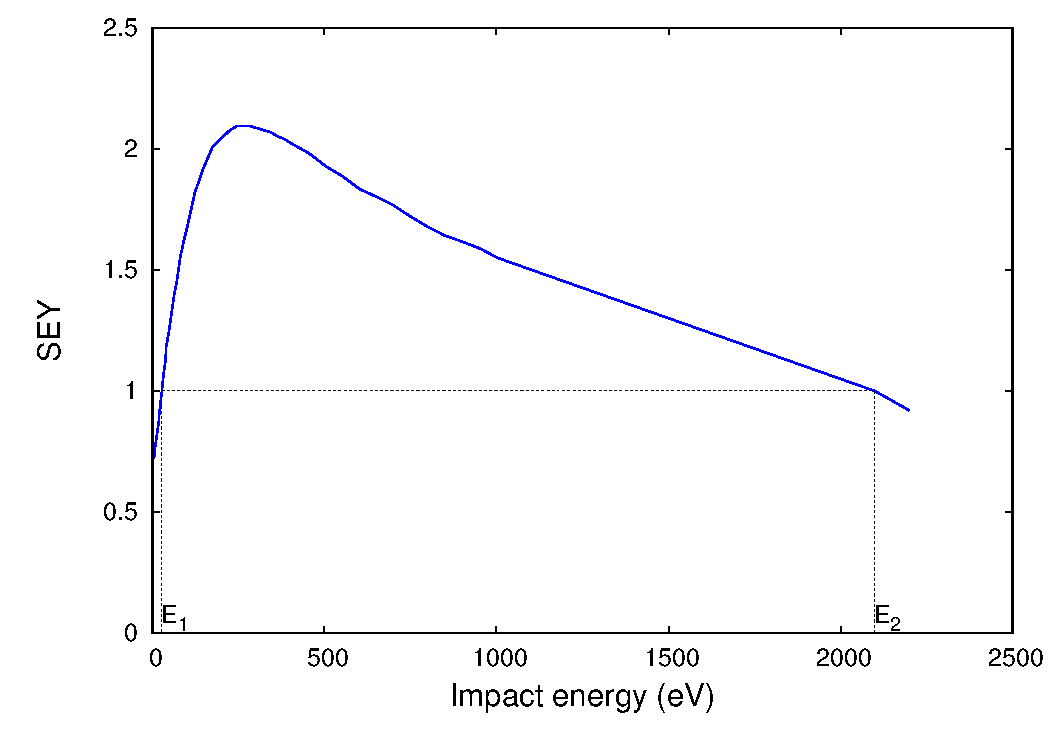
\includegraphics[width=0.8\linewidth,angle=0]{figures/Multipacting/SEY_curve.pdf}
  \caption{Typical SEY curve}
  \label{fig:typicalSEY}
 \end{center}
\end{figure}
Here, the horizontal axis is the energy of impacting electron, the vertical axis is the SEY value $\delta$, defined as \cite{Furman-Pivi}:
 \begin{equation}
\delta = \frac{I_s}{I_0} \label{eq:SEY}
\end{equation}
where $I_0$ is the incident electron beam current and $I_s$ is the secondary current, i.e., the electron current emitted from the surface. Usually the SEY value $\delta$ appeared in an SEY curve is the measured SEY with normal incident, i.e., the impacting electron is perpendicular to the surface. The energy $E_1$ and $E_2$ are the first crossover energy and the second crossover energy respectively, where the SEY value $\delta$ exceed and fall down to $\delta = 1$ at the first time. Obviously, only the energy range of $\delta>1$, i.e., $E \in (E_1,E_2)$ can contribute to multipacting.

Both Furman-Pivi's probabilistic secondary emission model \cite{Furman-Pivi} and Vaughan's formula based secondary emission model \cite{Vaughan} have been implemented in \opal and have been benchmarked \seesec{RunPP}.

The Furman and Pivi's secondary emission model calculates the number of secondary electrons that result from an incident electron of a given energy on a material at a given angle (see \figref{incident electrons}). For each of the generated secondary electrons the associated process: \emph{true secondary}, \emph{rediffused} or \emph{backscattered} is recorded, as is sketched in \figref{incident electrons}.
\begin{figure}
    \centering
    \scalebox{0.7} {
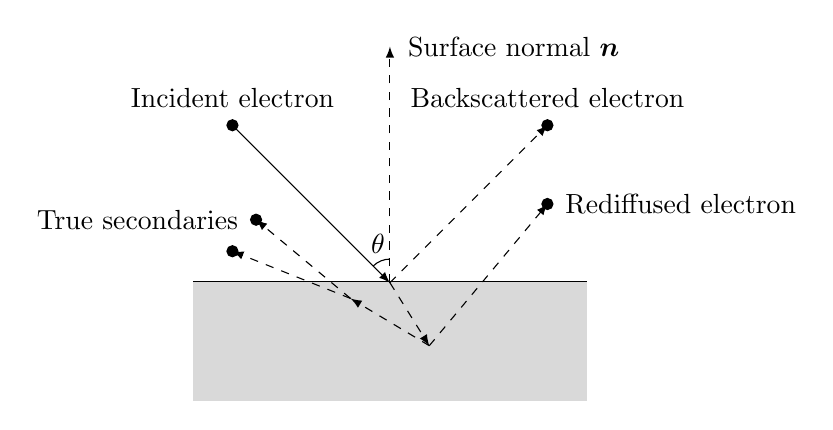
\begin{tikzpicture}
\usetikzlibrary{arrows}
\draw [very thick] (-2.5,0) -- (2.5,0);
\draw[gray!30,fill=gray!30] (-2.5,-1.5) rectangle (2.5,0); 
\draw [->,dashed,-latex] (0,0) -- (0,3);
%\node[below] (w) at (-0.15,0.5) {$\vec{w}$};
\node[right=3pt] (n) at (0,3) {Surface normal $\vec{n}$};
\path[draw=black,fill=black] (-2,2.0) circle (2pt);
\node[above=3pt] (electron) at (-2,2) {Incident electron};
\path[draw=black,fill=black] (2,2.0) circle (2pt);
\node[above=3pt] (electron1) at (2,2) {Backscattered electron};
\draw [->,-latex] (-2,2.0) -- (0,0);
\draw [dashed,->,-latex]  (0,0) -- (2,2.0);
\draw [dashed,->,-latex]  (0,0) -- (0.5,-0.8);
\draw [dashed,->,-latex]  (0.5,-0.8) -- (2,1);
\path[draw=black,fill=black] (2,1.0) circle (2pt);
\node[right=3pt] (electron1) at (2,1) {Rediffused electron};
\draw [dashed,->,-latex]  (0.5,-0.8) -- (-0.5,-0.2);
\draw [dashed,->,-latex] (-0.5,-0.2) -- (-2,0.4);
\draw [dashed,->,-latex] (-0.5,-0.2) -- (-1.7,0.8);
\path[draw=black,fill=black] (-2,0.4) circle (2pt);
\path[draw=black,fill=black] (-1.7,0.8) circle (2pt);
\node[left=3pt] (electron1) at (-1.7,0.8) {True secondaries};
\node[above] (theta) at (-0.15,0.25) {$\theta$};
\draw (0,0.3) arc (90:135:0.3);
\end{tikzpicture}
}
    % \includegraphics[width=3 in]{incident_diagram.pdf}
    \caption{Sketch map of the secondary emission process.}
    \label{fig:incident electrons}
\end{figure}
This model is mathematically self-consistent, which means that (1) when averaging over an infinite number of secondary-emission events, the reconstructed $\delta$ and $\uglyder{\delta}{E}$ are guaranteed to agree with the corresponding input quantities; (2) the energy integral of $\uglyder{\delta}{E}$ is guaranteed to equal $\delta$; (3) the energy of any given emitted electron is guaranteed not to exceed the primary energy; and (4) the aggregate energy of the electrons emitted in any multi-electron event is also guaranteed not to exceed the primary energy. This model contains built-in SEY curves for copper and stainless steel and the only thing user need to set is to choose the material type, i.e., copper or stainless steel, as long as the surface material of user's RF structure has the same SEY curve as built-in SEY curves.

Although a set of parameters in the model can be adjusted to model different SEY curves without breaking the above mentioned mathematical self-consistency, it is easier to use Vaughan's formula based secondary emission model if user has to model a different SEY curve.

The Vaughan's secondary emission model is based on a secondary emission yield formula \cite{Vaughan, VaughanRv}:
\begin{subequations}
\label{allequations}
\begin{eqnarray}
    \delta(E,\theta)&=&\delta_{max}(\theta)\cdot (v e^{1-v})^k,\ \text{for}\ v \le 3.6 \label{eq:VaughanA}
\\
\delta(E,\theta)&=&\delta_{max}(\theta)\cdot 1.125/v^{0.35},\ \text{for}\ v > 3.6 \label{eq:VaughanB}
\\
\delta(E,\theta)&=&\delta_0,\ \text{for}\ v \le 0 \label{eq:VaughanC}
\end{eqnarray}
\end{subequations}
where
\begin{eqnarray*}
v=\frac{\displaystyle E-E_0}{\displaystyle E_{max}(\theta)-E_0},
\end{eqnarray*}
\begin{eqnarray*}
k=0.56,\ \ \text{for}\ v<1,
\end{eqnarray*}
\begin{eqnarray*}
k=0.25,\ \ \text{for}\ 1<v\le{3.6},
\end{eqnarray*}
\begin{eqnarray*}
\delta_{max}(\theta)=\delta_{max}(0)\cdot (1+k_{\theta}\theta^2/2\pi),
\end{eqnarray*}
\begin{eqnarray*}
E_{max}(\theta)=E_{max}(0)\cdot (1+k_E\theta^2/2\pi).
\end{eqnarray*}
The secondary emission yield value for an impacting electron energy $E$ and incident angle $\theta$ w.r.t the surface normal is denoted as $\delta(E,\theta)$. Parameter $k_{\theta}$ and $k_E$ denotes the dependence on surface roughness. Both
should be assigned a default value of 1.0, which appears appropriate for typical dull surfaces in a working tube environment, and lower values down to zero or higher values, up to about 2.0, are only valid for specified cases \cite{Vaughan}. $E_{max}(0)$ is the impacting energy when incident angle is zero and secondary yield reaches its maximum value. $E_0$ is an adjustable parameter to make the first crossover energy be fitted to the experiment data \cite{FS}. $\delta_0$ is the user specified constant denote the SEY of low impacting energy.

The emission energy obeys the thermal energy distribution:
\begin{equation}
f(\epsilon) = \frac{\epsilon}{(k_BT)^2}exp\left(\frac{-\epsilon}{k_BT}\right) \label{eq:emienergy}
\end{equation}
The polar angles of emitted secondaries $\theta \in [0, \pi/2]$ are with probability density $\cos^{\alpha}\theta$, and the azimuthal angles $\phi \in [0, 2\pi]$ are with uniform probability density. These emission angles of the secondary electrons is relative to the local coordinate system which is centered at the collision point and whose $z$ axis is along the inward normal of the surface.

Motivated by the fact that the population of particles in simulation domain may continually grow exponentially and lead to tens of magnitude larger within limited simulation time steps, which may cause the exhaust of computing memory, a re-normalization of simulation particle number approach is also implemented. In each electron impacting events, instead of emitting the real number of simulation particles predicted by secondary emission models, this re-normalization approach emit only one particle, and the current of newly emitted particle will be the current of incident particle multiplied by SEY value $\delta$.
\clearpage
\section{Commands Related to Multipacting Simulation}
\label{sec:MultipactingCmd}
To perform multipacting simulation, a triangulated surface geometry defined in the  \keyword{GEOMETRY} command \seechp{geometry} must be specified and attached to the elements (currently only \keyword{RFCavity}, \keyword{ParallelPlate} and \keyword{Drift} elements are available for multipacting simulation).

A distribution array, containing \keyword{SURFACEEMISSION} and \keyword{SURFACERANDCREATE} type of distributions, defined in the \keyword{DISTRIBUTION} command must be attached to the
\keyword{GEOMETRY}. Users can use commands contained in \keyword{SURFACERANDCREATE} type of distribution to specify the position of initial \emph{seed} electrons. And commands within \keyword{SURFACEEMISSION} type of distribution can be used to customize the type and the parameters of secondary emission model in input file.

A summary of multipacting simulation related parameters are given in \tabref{Multipactingcmd}.

The following example shows the usage of the multipacting simulation related command.\\
\examplefromfile{examples/multipacting.in}

\begin{table}[ht] \footnotesize
  \begin{center}
    \caption{Multipacting Related Command Summary}
    \label{tab:Multipactingcmd}
    \begin{tabular}{|l|p{0.8\textwidth}|l|}
      \hline
      \tabhead{Command &Purpose (Default)}
      \hline
      \keyword{VW} \index{VW} & Velocity scalar in Maxwellian Dist (\SI{1.0}{\meter/\second})\\
      \keyword{VVTHERMAL} \index{VVTHERMAL} & Thermal velocity in Maxwellian Dist (\SI{7.268929821e5}{\meter/\second})\\
      \keyword{SECONDARYFLAG} \index{SECONDARYFLAG} & Secondary model type, 0:none, 1:Furman-Pivi, 2:Vaughan (\num{0})\\
      \keyword{NEMISSIONMODE} \index{NEMISSIONMODE} & Emit real No. secondaries or not (\keyword{TRUE})\\
      \keyword{VEZERO} \index{VEZERO} & SEY will be $\delta_0$, if energy is less than \keyword{VEZERO} in Vaughan's model (\SI{12.5}{\electronvolt})\\
      \keyword{VSEYZERO} \index{VSEYZERO} & $\delta_0$ in Vaughan's model (\num{0.5})\\
      \keyword{VSEYMAX} \index{VSEYMAX} & $\delta_{max}$ in Vaughan's model (\num{2.22})\\
      \keyword{VEMAX} \index{VEMAX} & Energy related to $\delta_{max}$ in Vaughan's model (\SI{165}{\electronvolt})\\
      \keyword{VKENERGY} \index{VKENERGY} & The roughness of surface for impact energy in Vaughan's model (\num{1.0}) \\
      \keyword{VKTHETA} \index{VKTHETA} & The roughness of surface for impact angle in Vaughan's model (\num{1.0}) \\
      \keyword{SURFMATERIAL} \index{SURFMATERIAL} & The material type for Furman-Pivi model, 0: copper; 1: stainless steel (\num{0})\\
      \hline
    \end{tabular}
  \end{center}
\end{table}

\clearpage
\section{Run Parallel Plate Benchmark}
\label{sec:RunPP}
\index{RunPP}
Both the Furman-Pivi's model and Vaughan's model have been carefully benchmarked in both re-normalize simulation particle approach and real simulation particles approach against a non-stationary multipacting theory \cite{nonstationary}. The \opal simulation results and the theory match very well \seefig{PPFurman-Pivi,PPVaughan}.
\begin{figure}[ht]
 \begin{center}
 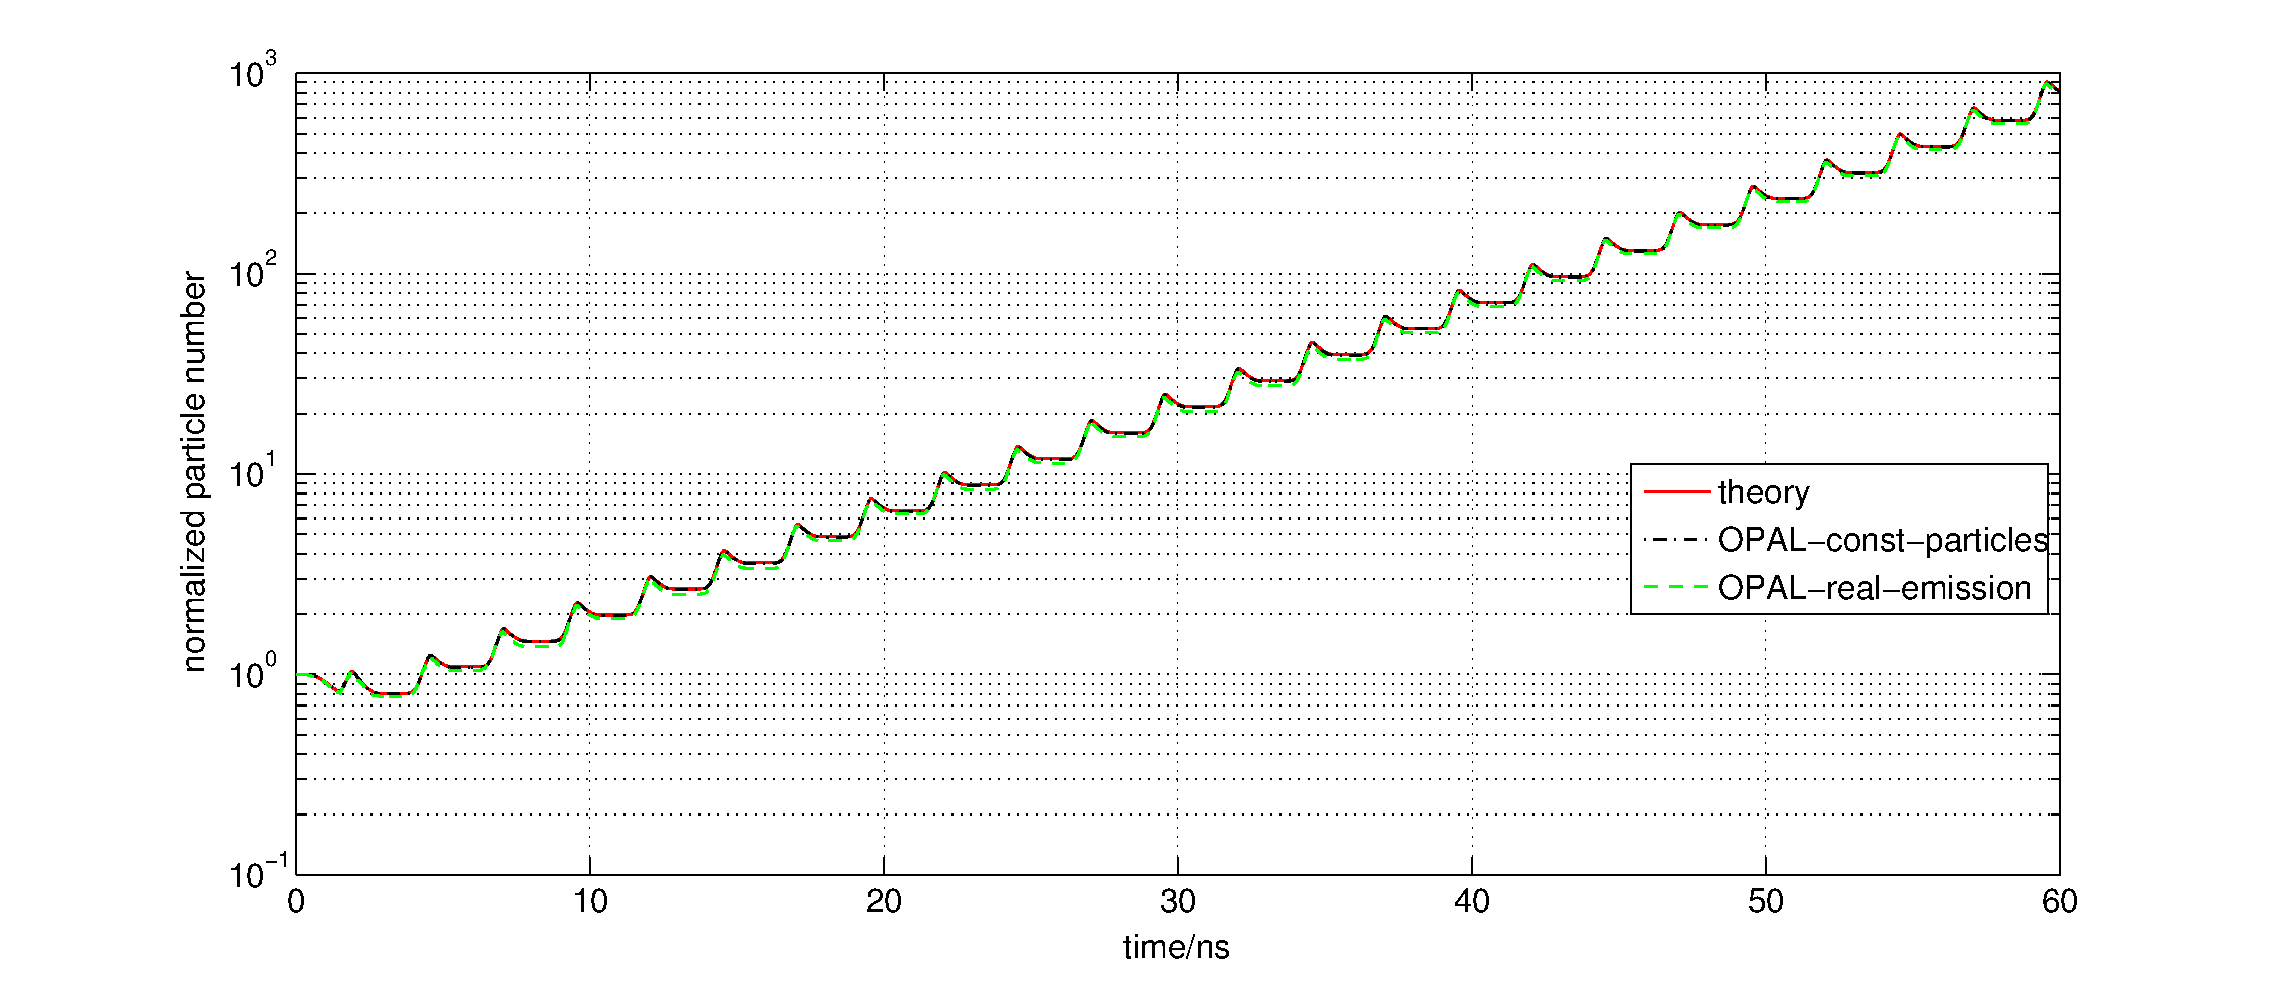
\includegraphics[width=1\linewidth,angle=0]{figures/Multipacting/const_particle_benchmark_FurmanPivi.pdf}
  \caption{Time evolution of electron number predicted by theoretical model and \opal simulation using Furman-Pivi's secondary emission model with both constant simulation particle approach and real emission particle approach at $f=\SI{200}{\mega\hertz}$, $V_0=\SI{120}{\volt}$, $d=\SI{5}{\milli\meter}$}
  \label{fig:PPFurman-Pivi}
 \end{center}
\end{figure}
\begin{figure}[ht]
 \begin{center}
 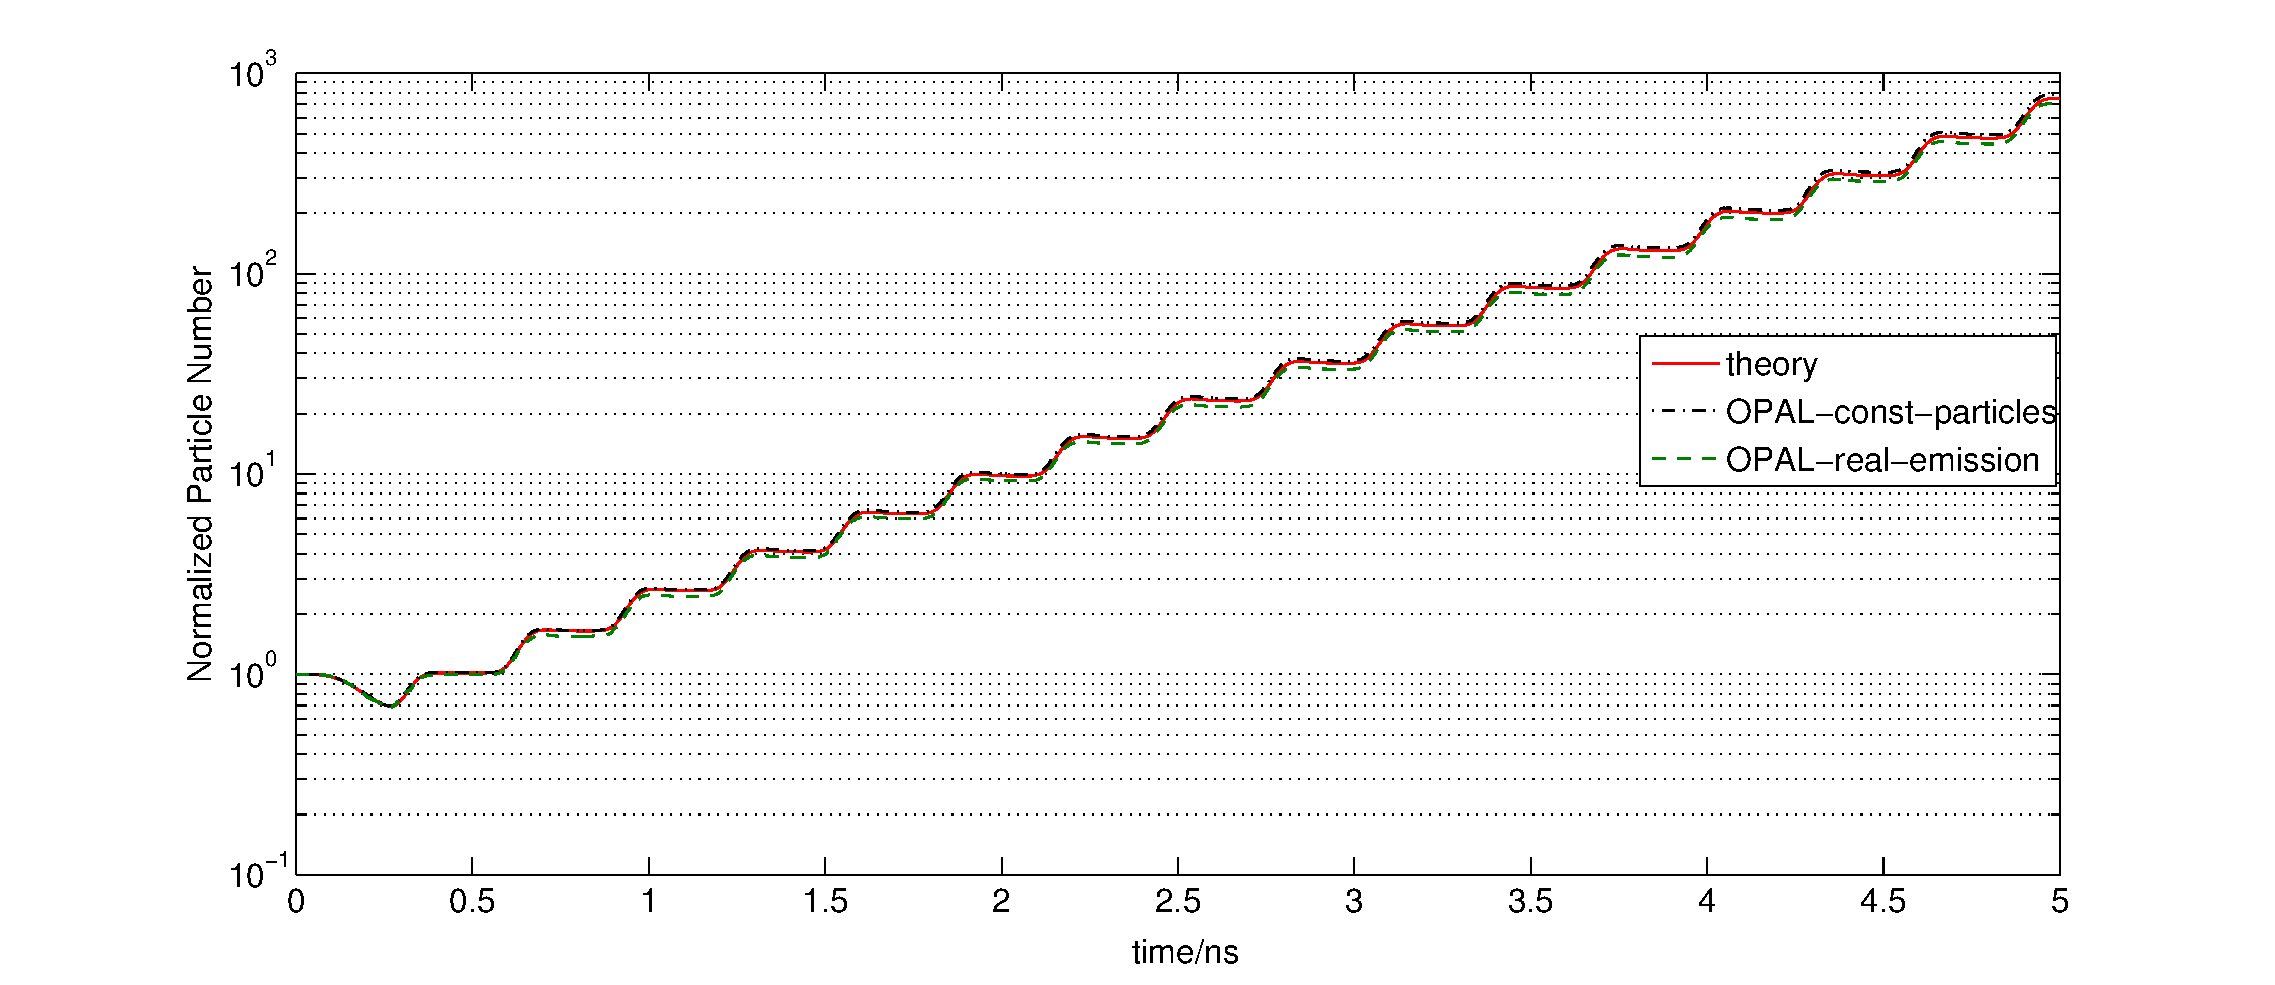
\includegraphics[width=1\linewidth,angle=0]{figures/Multipacting/const_particle_benchmark.pdf}
  \caption{Time evolution of electron number predicted by theoretical model and \opal simulation using Vaughan's secondary emission model with both constant simulation particle approach and real emission particle approach at $f=\SI{1640}{\mega\hertz}$, $V_0=\SI{120}{\volt}$, $d=\SI{1}{\milli\meter}$.}
  \label{fig:PPVaughan}
 \end{center}
\end{figure}

To run the parallel plate benchmark simulation, user need to set the option \keyword{PPDEBUG} in the input file $\mathbf{true}$. The input file and the geometry file needed by the parallel plate benchmark simulation can be found in the regression test folder.
\clearpage
\section{Post-Processing}
\label{sec:PostProcessing}
\index{Multipacting!PostProcessing}
In the general case (not only in multipacting simulations), \opal will dump the 6D phase space and statistical information of the particles in the simulation domain, into a \filename{h5} file. The dump frequency, i.e., after how many time steps the particle information will be saved can be specified with the option \keyword{PSDUMPFREQ}. Setting \keyword{Option, PSDUMPFREQ=1} dumps the information in each time step.

A utility tool \filename{h5ToVtk}  converts the \filename{h5} file to the Visualization Toolkit (VTK) legacy format. The number of VTK files equals to the number of time steps in \filename{h5} file. These VTK files together with a VTK file automatically generated by the geometry class of \opal which contains the geometry of the RF structure under study can be visualized using for example with Paraview \cite{paraview}. The animation and clip feature of Paraview is very useful to visualize the particle motion inside the RF structure.

For simulations involving the geometry (multipacting and field emission), \opal will also dump the position and current of incident particles into another \filename{h5} file with the name \filename{*\_Surface.h5}, where the asterisk stands for the base name of the user's \opal input file. If we need this surface loss data during post processing, we should specify the dump frequency in the option \keyword{SURFDUMPFREQ} with a positive integer in the \opal input file, otherwise, the default value of the option is \keyword{SURFDUMPFREQ=-1}, and the \filename{*\_Surface.h5} will not be generated. Another utility tool \filename{h5SurfaceVtk}  convert the \filename{*\_Surface.h5}  file to VTK files. For multipacting simulation, these VTK files can be used to visualize the \emph{hot spots} of the RF structure where multipacting happens.

The above mentioned utility tools are based on H5hut library, and will soon be available in the distribution.

Some of the boundary geometry related simulations, like the multipacting simulation using re-normalizing particle number approach, or dark current simulations where the current of field emitted particles from a single triangle has been re-normalized as the model predicted current has exceeded the user defined upper limit, the current (weight) of simulation particles varies and each simulation particle stands for more physical particles than the initial simulation particles. In these cases, instead of using simulation particles, we count the number of \emph{effective particles} defined as the ratio of total current in simulation over the current of a single initial particle.

An ASCII file named \filename{Part\_statistics.dat} containing the simulation time, the number of impacts and associated total SEY value as well as the number of \emph{effective particles} in each time step. This makes the analysis of the time evolution of particle density feasible with  tools like GNUPLOT.


%----------- Footer control ------------------
\ifthenelse{\boolean{FullOPALManual}}
{
  %do nothing
}
% else (for individual document creation)
{
\appendix
\printbibliography
\end{document}
}
%---------------------------------------------